\documentclass[14pt, a4paper]{extarticle}
\usepackage[utf8]{inputenc}
\usepackage[russian]{babel}
\usepackage{graphicx}
\usepackage{float}
\usepackage{caption}
\usepackage{subcaption}
\usepackage{url}
\usepackage{multirow}
\usepackage{mathtools}
\usepackage{amsmath}
\usepackage[left=2cm,right=2cm,bottom=3cm,top=2cm]{geometry}
\usepackage{multirow}

\DeclarePairedDelimiter{\abs}{\lvert}{\rvert}

\linespread{1.25}

\begin{document}

\thispagestyle{empty}

\begin{center}
\ \vspace{-3cm}

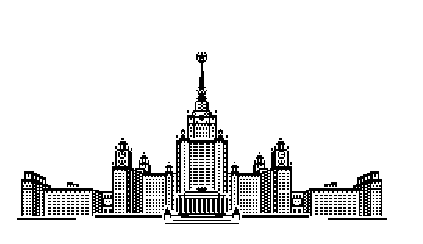
\includegraphics[width=0.5\textwidth]{img/msu.eps}\\
{Московский государственный университет имени М.В.~Ломоносова}\\
Факультет вычислительной математики и кибернетики\\
Кафедра интеллектуальных информационных технологий

\vspace{5cm}

{\Large Бородин~Григорий~Романович}

\vspace{1cm}

{\Large\bfseries
Сегментация структур сердца на изображениях магнитно-резонансной томографии с применением нейросетевых алгоритмов\\}

\vspace{1cm}

{\large ДИПЛОМНАЯ РАБОТА}
\end{center}

\vfill

\begin{flushright}
  \textbf{Научный руководитель:}\\
  к.ф.-м.н.\\
  О.В.~Сенюкова
\end{flushright}

\vfill

\begin{center}
Москва, 2018
\end{center}

\enlargethispage{4\baselineskip}

%\newpage
%\noindent 
%\textbf{Прогнозирование степени дискомфорта зрителей при просмотре стереоскопического фильма по его техническому качеству}\\
%Анциферова Анастасия\\
%В настоящее время большое количество фильмов производится в стереоскопическом формате. Несмотря на развитие технологии стереосъёмки, даже в высокобюджетных фильмах встречаются искажения, которые вызывают головную боль и дискомфорт у зрителей во время просмотра. Существующие методы автоматического контроля качества стереофильмов способны обнаружить такие искажения, однако оценка дискомфорта, вызванного отдельными искажениями, будучи сложной задачей, вызывает трудности. Данная работа посвящена исследованию влияния геометрических, цветовых и временных несоответствий между ракурсами стереофильма на уровень дискомфорта зрителя. В серии экспериментов было проведено анкетирование 302 человек по результатам просмотра фрагментов художественных стереофильмов с искусственно добавленными дозированными искажениями. Анкета состояла из вопросов о степени визуального дискомфорта, причиняемого каждым из продемонстрированных фрагментов, а также о поле и возрасте участника. Анализ полученных данных выявил зависимость между интенсивностью движения в сцене и степенью дискомфорта, причиняемой фрагментами с временным несоответствием.

%\noindent 
%\\[1mm]
%\textbf{Forecasting of viewers' discomfort degree when watching stereoscopic movie by its technical quality}\\
%Antsiferova Anastasiia\\
%Nowadays a large number of movies are produced in stereoscopic format. Despite stereo technology improvement, stereoscopic artifacts that cause headache and discomfort in viewers can still be found even in high-budget films. Existing automatic quality control algorithms are able to detect such distortions, however, they do not take into account a viewer's subjective perception of different artifacts. In this research the influence of geometric, color and temporal discrepancies in the stereo pair on a viewer's discomfort is explored. A series of experiments with passive stereo cinema technology was conducted. 60 video sequences from stereoscopic movies with artificially added distortions were demonstrated to the audience. 302 subjects took part in the experiments. During the analysis of the obtained data, the dependencies between the degree of spectators' discomfort and the intensity of distortions were revealed.

\clearpage
\newpage

\renewcommand{\contentsname}{Содержание}
\tableofcontents
\clearpage
\newpage

\section{Введение}
Медицина - широкий раздел биологии, который занимается спектром задач, связанным с диагностикой, лечением и профилактикой заболеваний, а также с сохранением и укреплением здоровья и трудоспособности людей. 

Благодаря современным технологиям стало возможным обследование огромного количества людей в автоматическом режиме. Это, в свою очередь, позволило диагностировать болезни на ранней стадии, улучшить профилактику заболеваний, сохранить жизнь многим людям.

В современном мире можно очень легко и быстро собрать детализированную информацию о пациенте, проанализировать ее и быстро среагировать на любое отклонение от нормы. Основные способы получения информации о пациенте включают: рентгенографию, компьютерную томографию, маммографию, магнитно-резонансная томография (МРТ), ультразвуковое исследование (УЗИ), а также различные виды анализов. Такое разнообразие показателей позволяет сильно упростить исследования с помощью автоматизации процесса.

Людей, которые профессионально занимаются медициной, очень мало, потому что обучение по этой специальности занимает очень много времени. По этой причине особенно важно максимально освободить этих людей от рутинной работы, не говоря уже о том, что человек легко может сделать ошибку.

Технологии анализа больших данных и машинного обучения позволяют построить эффективные модели, которые смогут решать самые разные задачи: по результатам анализов можно предсказать вероятности присутствия той или иной болезни, а по снимкам рентгена или мрт можно автоматически выявить отклонения размеров органов или их положения от нормы. Автоматизация решения этих задач позволяет в разы ускорить процесс диагностирования заболеваний, а также даёт врачам возможность заниматься более сложными случаями и спасать больше людей.

Целью этой работы является построение алгорима, решающего задачу сегментации снимков МРТ сердца. Результат решения такой задачи позволяет определить точное положение сердца относительно других органов и тканей, оценить размер сердца в заданной фазе и даже построить объемную модель сердца пациента.

Среди методов сегментации выделяют автоматические и полуавтоматические. 

Для решения задачи мы будем использовать сверточные нейронные сети.


\clearpage
\newpage
\section{Постановка задачи}

Целью данной работы является построение алгоритма, который решает задачу сегментации снимков МРТ сердца. Задача сегментации заключается в том, чтобы определить, какие части изображения принадлежат целевому объекту, а какие нет. 

\subsection{Входные данные}

Каждый набор данных разделен на 3 части: 

\begin{itemize}
  \item данные для обучения
  \item данные для валидации
  \item данные для тестирования
\end{itemize}

Данные для обучения и валидации — это пары $(\hat{X}_{train},\hat{Y}_{train})$ и $(\hat{X}_{val},\hat{Y}_{val})$, где $\hat{X}_{train} = \{\hat{x}_{train,i}\},i\in{}\overline{1,n_{train}}$ и $\hat{X}_{val} = \{\hat{x}_{val,i}\},i\in{}\overline{1,n_{val}}$ соответственно — 2 упорядоченных набора матриц, каждый элемент каждой из которых представляет собой интенсивность соответствующего участка на снимке МРТ сердца, $\hat{Y}_{train}$ и $\hat{Y}_{val}$ соответственно — 2 упорядоченных множеств пар $(x_{i},y_{i}), i = \overline{1,m}$, определяющее \mbox{$m$-угольник} — выделенный экспертом контур сердца.

Данные для тестирования — упорядоченный набор матриц $\hat{X}_{test} = \{\hat{x}_{test,i}\},i\in{}\overline{1,n_{test}}$, каждый элемент каждой из которых представляет собой интенсивность соответствующего участка на снимке МРТ сердца, для которого необходимо предсказать контур искомого объекта.

\subsection{Формальная постановка задачи}

Чтобы использовать нейронную сеть для решения задачи, преобразуем каждый набор $\hat{X},\hat{X}\in{}\{\hat{X}_{train},\hat{X}_{val},\hat{X}_{test}\}$ к соответствующему новому упорядоченному набору $X,X\in{}\{X_{train},X_{val},X_{test}\}$, каждый элемент которого — матрица $R^{n*n}$, каждый элемент которой, в свою очередь, представляет собой нормализованную интенсивность соответствующего участка на снимке МРТ сердца. 

Аналогично, преобразуем каждый набор $\hat{Y},\hat{Y}\in{}\{\hat{Y}_{train},\hat{Y}_{val}\}$ в соответствующий упорядоченный набор $Y,Y\in{}\{Y_{train},Y_{val}\}$, каждый элемент которого — матрица $R^{n*n}$, каждый элемент которой, в свою очередь, является $1$ или $0$, в зависимости от того, принадлежит ли соответствующий пиксель заданному \mbox{$m$-угольнику} или нет.

Таким образом, исходная задача сводится к задаче бинарной классификации каждого пикселя входного изображения — либо пиксель принадлежит объекту, либо нет. На вход алгоритму подаются нормализованные матрицы снимков МРТ, а на выходе алгоритма получается матрица, каждый элемент которой показывает вероятность принадлежности соответствующего пикселя объекту. Выход алгоритма затем сравнивается с разметкой с помощью различных метрик.

\subsection{Метрики}

Чтобы оценить качество сегментации, введем метрики оценки качества сегментации. Результат сегментации можно представить либо как область пикселей, либо как контур вокруг этой области. 

Индекс Дайса (Dice index) позволяет сравнить 2 области:

$Dice(A,B) = \frac{2|A\cap{}B}{|A| + |B|}$

Индекс Джаккарда (Jaccard index) — еще одна метрика для сравнения областей:

$J(A,B) = \frac{|A\cap{}B|}{|A\cup{}B}$

Метрика Хаусдорфа (Hausdorff distance) позволяет оценить схожесть контуров:

$\mathrm{d}_{H}(A,B)=\max\left\{\sup_{a\in{}A}\inf_{b\in{}B}\mathrm{d}(a,b),\sup_{b\in{}B}\inf_{a\in{}A}\mathrm{d}(a,b)\right\}$

Чтобы посчитать индекс Джаккарда или индекс Дайса, необходимо предварительно преобразовать экспертную разметку



\clearpage
\newpage
\section{Обзор существующих методов}

Существует много алгоритмов для решения задачи семантической сегментации или задачи поиска контура. Сюда входят, в том числе, методы активного контура~\cite{snakes}, сегментация с помощью кластеризации~\cite{clustering_segm} и нейросетевые методы~\cite{fcn},~\cite{unet},~\cite{gridnet}.

\subsection{Простая сверточная модель}

Простая сверточная модель~\cite{fcn_1_layer_upsample} была разработана на основе сверточных нейронных сетей для классификации. Отличие состоит в том, что в сетях для класификации последний слой softmax~\cite{classification_loss} преобразует высокоуровневые признаки, полученные последовательным применением сверток в вероятности принадлежности к классам, а~для~сегментации сначала используется upsampling слой, который преобразует высокоуровневые признаки в~изображение размером с~исходное, которое описывает, где именно находится объект. Каждый сверточный блок состоит из~нескольких слоев, расположенных друг за~другом, как описано в~таблице~\ref{tab:conv_block}.

\begin{table}[b]
  \begin{center}
    \begin{tabular}{ c }
      \hline
      сверточный слой с~ядром~3x3           \\ \hline
      mvn слой                              \\ \hline
      сверточный слой с~ядром~3x3           \\ \hline
      mvn слой                              \\ \hline
      \dots                                 \\ \hline
      maxpool слой с~ядром~2x2 и~шагом~2    \\ 
      \hline
    \end{tabular}
    \caption{Структура сверточного блока} \label{tab:conv_block}
  \end{center}
\end{table}

Такая структура часто используется в нейронных сетях, потому что позволяет ускорить сходимость и~уменьшить количество вычислений при~сохранении точности. Сверточные слои обеспечивают вычисление высокоуровневых признаков с помощью применения фильтров к входному изображению. Maxpool слои позволяют уменьшить сложность вычислений, и оставить самую важную информацию, полученную из сверточных слоев. Слой dropout помогает избежать переобучения~(\cite{dropout}). 

\subsection{Модель c обратной сверткой}
 
Модель с обратной сверткой~\cite{fcn} более сложная. Она состоит из~нескольких сверточных блоков и~нескольких обратных сверточных блоков. Каждый блок, в~свою очередь, состоит из~нескольких сверточных слоев с~функцией активации relu и~maxpool~слоя. 

Всего в~нейронной сети 3~сверточных блока и~1~блок без~maxpool слоя. Они идут подряд, и~каждый следующий на~выходе дает в~2~раза больше фильтров. 

Структура обратного блока, напротив, нелинейная:

\begin{itemize}
  \item обратный сверточный слой с~ядром~3x3 и~шагом~2,
  \item сверточный слой с~ядром~1х1 и~шагом~1, который вычисляется от~предыдущего mvn~слоя,
  \item слой, который вычисляет среднее арифметическое из~первых двух слоев блока.
\end{itemize}

Всего в нейронной сети 3~обратных блока. Количество фильтров в каждой свертке обратного блока равно количеству классов. Если же класса всего~2, то мы задаем на выходе 1~фильтр и~в~конце используем функцию активации sigmoid, вычисляя ошибку при этом с~помощью индекса Дайса. В данной работе во~всех случаях используется только 2~класса.

Обозначим сверточный блок с~$k$~свертками и~$n$~фильтрами как~$conv(k,n)$. Обозначим обратный сверточный слой, который получает на одном из входов $n$~фильтров как~$deconv(n)$. Обозначим слой dropout регуляризации с параметром $p$ как $dropout(p)$. Архитектура всей сети описана в таблице \ref{tab:fcn}.

\begin{table}
  \begin{center}
    \begin{tabular}{ c }
      \hline
      вход                              \\ \hline
      $conv(3,64)$                      \\ \hline
      $conv(4,128)$                     \\ \hline
      $conv(4,256)$                     \\ \hline
      $droupout(0.5)$                   \\ \hline
      $conv(4,512)$ без maxpool слоя    \\ \hline
      $droupout(0.5)$                   \\ \hline
      $deconv(512)$                     \\ \hline
      $deconv(256)$                     \\ \hline  
      $deconv(128)$                     \\ \hline      
      sigmoid активация                 \\
      \hline
    \end{tabular}
    \caption{Архитектура модели с обратной сверткой} \label{tab:fcn}
  \end{center}
\end{table}

Чтобы сеть сходилась устойчиво, после каждой свертки используется mvn слой~(\cite{batch_norm}). Обратные сверточные слои позволяют получить карту вероятностей принадлежности входных пикселей объекту в~зависимости от~контекста из~высокоуровневых признаков, вычисленных сверточными слоями. Каждый блок обратной свертки связан не только с предыдущим блоком обратной свертки, но и с соответствующим по размеру сверточным блоком, для того, чтобы обеспечить сходимость сети. Несколько обратных слоев позволяют сгладить резкие переходы на~выходной карте вероятностей и~получить более точные предсказания. В~обратных блоках учитываются выходы соответствующих mvn слоев прямых блоков, чтобы увеличить скорость обучения. Этот прием очень похож на~residual блоки в~\cite{resnet}.

\subsection{U-Net}

Архитектура U-Net \cite{unet} основана на идеях, перечисленных при описании более простых моделей. Здесь также используются прямые и обратные блоки. 

Каждый прямой блок модели U-Net состоит из 2-х сверточных слоев с ядром 3х3 и функцией активации relu. В обратных блоках используются простые upsampling слои для получения изображения из высокоуровневых сетей. Кроме того, в обратных блоках присутствует merge слой, который конкатенирует выход соответствущего по размеру прямого блока и выход предыдущего обратного блока. Такое решение позволяет получать быструю сходимость сети, так как при алгоритме обратного распространения ошибки, последняя не затухает, а сразу передается на сверточные блоки. Помимо этого, точность модели улучшается за счет увеличения количества параметров.   

\subsection{GridNet}

Модель Gridnet \cite{gridnet} являтся развитием модели U-Net.

\clearpage
\newpage
\section{Исследование и построение решения задачи}

Решение задачи проходило в несколько этапов:

\begin{itemize}
  \item реализация существующих моделей,
  \item вычисление метрик каждой модели на каждом наборе данных,
  \item анализ результатов,
  \item построение новой модели и подбор параметров,
  \item сравнение результатов новой модели и существующих.
\end{itemize}

\subsection{Наборы данных}

\paragraph{Sunnybrook}

Набор содержит снимки 45 пациентов. У разных пациентов, 
снимки которых присутствуют в наборе, разное состояние здоровья сердца: 
у некоторых заболеваний~нет, у~остальных — разные виды заболеваний. 
Для~обучения присутствует экспертная разметка эндокарда, эпикарда 
и~сосочковых мышц. Набор разделен на 3~части по~15~пациентов 
в~каждом: часть для обучения, для валидации и~для~тестирования.

\paragraph{LVSC}

Набор содержит снимки 200 пациентов. Набор разделен на 2 части пополам: часть для обучения и~часть для~валидации. У всех пациентов присутствует ишемическая болезнь сердца и коронарная недостаточность.

\paragraph{RVSC}

Набор состоит из 48 снимков пациентов с разными заболеваниями сердца. Данные разделены на 3 части: одна для обучения и две для тестирования. Экспертная разметка присутствует только для части для обучения.

\subsection{U-Net с растянутой сверткой}

Для построения собственного решения были проанализированы существующие подходы 
и~нейронные сети для решения задачи семантической сегментации и выделения контура сердца. 
В этой работе предложена своя архитектура сети, решающая эту задачу.

За основу была взята модель U-Net, потому что она дает хороший результат. 
Идея архитектуры в~том, чтобы~заменить последовательные свертки в~U-Net 
на~последовательные растянутые свертки. В оригинальном~U-Net в~каждом блоке 
присутствует 2~сверточных слоя с~ядром~3x3 и~затем maxpool~слой. В~предложенной 
модели также используется 2~сверточных слоя, но~второй из~них в~каждом блоке 
вычисляется с~растяжением~2, то~есть~эффективное ядро свертки будет 5x5. 

\newpage

Размер контекста входного изображения в U-Net 140x140~\eqref{eq:unet_influence}, а~размер контекста предложенной архитектуры — 202x202~\eqref{eq:dilated_unet_influence}. Это существенно уменьшает возможность появления артефактов и ошибок второго рода.

\begin{equation} 
\label{eq:unet_influence}
1-3-5:10-12-14:28-30-32:64-66-68:136-138-140
\end{equation}
\begin{equation} 
\label{eq:dilated_unet_influence}
1-5-7:14-18-20:40-44-46:92-96-98:196-200-202
\end{equation}

Схемы~\eqref{eq:unet_influence}~и~\eqref{eq:dilated_unet_influence} показывают, как увеличивается контекст при прохождении через сверточные и maxpool слои архитектуры U-Net~и~U-Net с~растянутой сверткой соответственно. Например, запись $5-7$ означает, что при прохождении через сверточный слой контекст увеличился с 5х5 до 7х7, а~запись $20:40$ означает, что при прохождении через maxpoool слой контекст увеличился с 20x20 до 40х40.

\clearpage
\newpage
\section{Описание практической части}

Проект был~реализован на~языке Python~3. Для реализации моделей использовался фреймворк tensorflow и~библиотекa keras. Наборы данных были получены в формате DICOM, поэтому для распаковки данных использовалась соответствующая библиотека dicom. Обработка данных в памяти осуществлялось с помощью библиотеки numpy. Для работы с изображениями использовалась библиотека OpenCV. Аугментация данных реализована с помощью встроенных в~keras средств для генерации и преобразования изображений налету ImageDataGenerator. Для всех моделей использовалось одинаковое количество эпох. Обучение и тестирование было реализовано с помощью обертки keras, которая позволяет использовать scikit-learn API с унифицированным интерфейсом для обучения, применения и проверки точности модели.

Решение задачи проходило в несколько этапов:

\begin{itemize}
  \item Реализация существующих моделей,
  \item Вычисление метрик каждой модели на каждом наборе данных,
  \item Анализ результатов
  \item Построение новой модели и подбор параметров
  \item Сравнение результатов новой модели и существующих
\end{itemize}


\clearpage
\newpage
\section{Заключение}

По таблицам~\ref{tab:lvsc_results},~\ref{tab:rvsc_results},~\ref{tab:sunnybrook_results} видно, что предложенная архитектура показывает хорошие результаты при~сравнительно небольшом размере сети. В случае, если не нужно сильно экономить место и память, и для решения задачи можно позволить себе сеть по количеству параметров больше U-Net, то имеет смысл использовать предложенную в этой статье архитектуру. 

\begin{table}[h]
  \begin{center}
    \caption{Результаты на наборе данных LVSC} \label{tab:lvsc_results}
    \begin{tabular}{ |c||*{3}{c|} }
      \hline
      \multirow{2}{*}{Метод}      & Количество   & \multicolumn{2}{c|}{Индекс Дайса} \\ \cline{3-4}
                                  & параметров   & Endocardium   & Epicardium        \\ \hline
      \hline
      FCN                         & $\sim11$~млн & 0.90          & 0.89              \\ \hline
      U-Net                       &  $\sim2$~млн & 0.92          & \textbf{0.90}     \\ \hline
      GridNet                     &  $\sim8$~млн & \textbf{0.93} & \textbf{0.90}     \\ \hline
      U-Net с~растянутой сверткой &  $\sim4$~млн & 0.92          & 0.88              \\ 
      \hline
    \end{tabular}

    \vspace{0.6cm}
    
    \caption{Результаты на наборе данных RVSC} \label{tab:rvsc_results}
    \begin{tabular}{ |c||*{3}{c|} }
      \hline
      \multirow{2}{*}{Метод}      & Количество   & \multicolumn{2}{c|}{Индекс Дайса} \\ \cline{3-4}
                                  & параметров   & Endocardium   & Epicardium        \\ \hline
      \hline
      FCN                         & $\sim11$~млн & 0.84          & \textbf{0.86}     \\ \hline
      U-Net                       &  $\sim2$~млн & 0.79          & 0.77              \\ \hline
      GridNet                     &  $\sim8$~млн & 0.82          & 0.81              \\ \hline
      U-Net с~растянутой сверткой &  $\sim4$~млн & \textbf{0.85} & 0.83              \\ 
      \hline
    \end{tabular}

    \vspace{0.6cm}
    
    \caption{Результаты на наборе данных Sunnybrook} \label{tab:sunnybrook_results}
    \begin{tabular}{ |c||*{3}{c|} }
      \hline
      \multirow{2}{*}{Метод}      & Количество   & \multicolumn{2}{c|}{Индекс Дайса} \\ \cline{3-4}
                                  & параметров   & Endocardium   & Epicardium        \\ \hline
      \hline
      FCN                         & $\sim11$~млн & 0.92          & \textbf{0.96}     \\ \hline
      U-Net                       &  $\sim2$~млн & \textbf{0.93} & 0.94              \\ \hline
      GridNet                     &  $\sim8$~млн & 0.90          & 0.93              \\ \hline
      U-Net с~растянутой сверткой &  $\sim4$~млн & 0.91          & \textbf{0.96}     \\ 
      \hline
    \end{tabular}
  \end{center}
\end{table}




\clearpage
\newpage

\renewcommand{\bibname}{Список литературы}
\addcontentsline{toc}{section}{\bibname}

\bibliographystyle{gost71s}
\bibliography{references}{}

\end{document} 